%----------------------------------------------------------------------------------------
% METADATA BLOCK (YAML)  — see inbox/README.md for every field
%----------------------------------------------------------------------------------------
% uid: ""
% school: "lycee"
% level: "3eme"
% section: "Mathématiques"
% chapter: "Produit scalaire dans le plan"
% title: "Euler et Poncelet : OI² = R² − 2Rr et sa réciproque"
% difficulty: "Difficile"
% tags: ["euler", "poncelet", "cercle-inscrit", "puissance-d-un-point", "triangle"]
% provenance: "adapted"
% batch: "2026-11-20-defis-geometrie-A"
%----------------------------------------------------------------------------------------

% ---STATEMENT---
\textbf{Partie A : la formule d'Euler.}
Soit $ABC$ un triangle, $\mathcal C$ son cercle circonscrit (centre $O$, rayon $R$), $I$ le centre de son cercle inscrit (rayon $r$). La droite $(AI)$ recoupe $\mathcal C$ en $M$. On note $\widehat{BAC}=2\alpha$.

% alt: Triangle ABC inscrit dans le cercle de centre O, cercle inscrit de centre I, la droite (AI) recoupe le cercle en M
\begin{center}
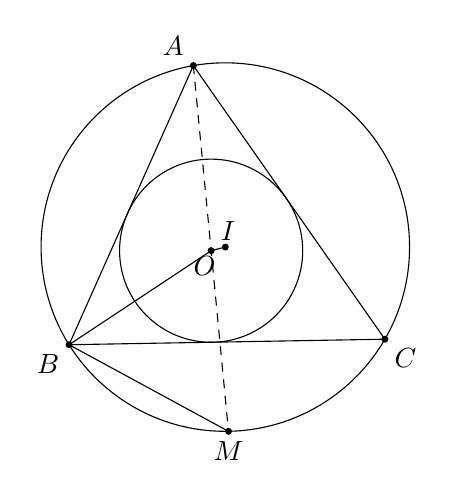
\begin{tikzpicture}[scale=0.9,line cap=round,line join=round,>=stealth]
\draw (0,0) circle (2.6);
\draw (-0.2,-0.051) circle (1.292);
\draw (-0.451,2.561) -- (-2.205,-1.378) -- (2.252,-1.3) -- cycle;
\draw[dashed] (-0.451,2.561) -- (0.045,-2.6);
\draw[thin] (0,0) -- (-0.2,-0.051);
\draw[thin] (-2.205,-1.378) -- (0.045,-2.6);
\draw[thin] (-2.205,-1.378) -- (-0.2,-0.051);
\fill(-0.451,2.561) circle (1.4pt) node[above left] {$A$};
\fill(-2.205,-1.378) circle (1.4pt) node[below left] {$B$};
\fill(2.252,-1.3) circle (1.4pt) node[below right] {$C$};
\fill(0.045,-2.6) circle (1.4pt) node[below] {$M$};
\fill(-0.2,-0.051) circle (1.4pt) node[above right] {$I$};
\fill(0,0) circle (1.4pt) node[below left] {$O$};
\end{tikzpicture}
\end{center}

\begin{enumerate}
  \item Montrer que $MB=MI$ (on calculera les angles $\widehat{MBI}$ et $\widehat{MIB}$).
  \item Montrer que $MB=2R\sin\alpha$ et que $AI=\dfrac{r}{\sin\alpha}$.
  \item En considérant la puissance de $I$ par rapport à $\mathcal C$ (on rappelle que, pour toute corde $[UV]$ de $\mathcal C$ passant par $I$, $IU\cdot IV=R^2-OI^2$), montrer que \textbf{$OI^2=R^2-2Rr$}.
\end{enumerate}

\textbf{Partie B : la réciproque (porisme de Poncelet).}
Soient un cercle $\mathcal C$ de centre $O$ et de rayon $R$ et un cercle $\gamma$ de centre $I$ et de rayon $r$ tels que $OI^2=R^2-2Rr$. Soit $A$ un point quelconque de $\mathcal C$. Les tangentes à $\gamma$ issues de $A$ recoupent $\mathcal C$ en $B$ et $C$.
\begin{enumerate}
  \item Soit $M$ le second point d'intersection de $(AI)$ avec $\mathcal C$ et $\alpha$ l'angle entre $(AI)$ et chacune des deux tangentes. Montrer que $MB=MC=MI$.
  \item Montrer que $I$ est le centre du cercle inscrit dans $ABC$ et que \textbf{$(BC)$ est tangente à $\gamma$}.
  \item En déduire que, pour tout point $A$ de $\mathcal C$, il existe un triangle de sommet $A$ inscrit dans $\mathcal C$ et circonscrit à $\gamma$ : il y en a donc une infinité.
\end{enumerate}

% ---SOLUTION---
\textbf{Partie A.}
\begin{enumerate}[itemsep=14pt]
  \item\leavevmode
  \begin{prop}[Angles inscrits et angle extérieur]
  Deux angles inscrits qui interceptent le même arc sont égaux. Dans un triangle, un angle extérieur est la somme des deux angles intérieurs non adjacents.
  \end{prop}
  Notons $\widehat{ABC}=2\beta$. Comme $I$ est sur les bissectrices, $\widehat{BAM}=\widehat{MAC}=\alpha$ et $\widehat{IBC}=\widehat{IBA}=\beta$.

  \emph{Angle $\widehat{MBI}$ :} $\widehat{MBC}=\widehat{MAC}=\alpha$ (angles inscrits qui interceptent l'arc $MC$). Donc
  \[\widehat{MBI}=\widehat{MBC}+\widehat{CBI}=\alpha+\beta.\]
  \emph{Angle $\widehat{MIB}$ :} c'est un angle extérieur du triangle $ABI$ : $\widehat{MIB}=\widehat{IAB}+\widehat{IBA}=\alpha+\beta$.

  Le triangle $MBI$ a deux angles égaux : il est isocèle de sommet $M$. Donc \ib{$MB=MI$}.

  \item Dans le triangle $ABM$ inscrit dans $\mathcal C$ :
  \begin{prop}[Loi des sinus]
  Dans un triangle inscrit dans un cercle de rayon $R$, chaque côté vaut \ib{$2R\sin(\text{angle opposé})$}.
  \end{prop}
  Le côté $MB$ est opposé à $\widehat{BAM}=\alpha$ : \ib{$MB=2R\sin\alpha$}.

  La distance de $I$ à $(AB)$ est $r$ et $(AI)$ fait un angle $\alpha$ avec $(AB)$ : $r=AI\sin\alpha$, donc \ib{$AI=\dfrac r{\sin\alpha}$}.

  \item $I$ est à l'intérieur de $\mathcal C$ et $[AM]$ est une corde passant par $I$ : $IA\cdot IM=R^2-OI^2$.

  Or $IM=MB=2R\sin\alpha$ et $IA=\dfrac r{\sin\alpha}$ :
  \[R^2-OI^2=\dfrac r{\sin\alpha}\times2R\sin\alpha=2Rr.\]
  Donc \ib{$OI^2=R^2-2Rr$}. $\blacksquare$
\end{enumerate}

\textbf{Partie B.}
\begin{enumerate}[itemsep=14pt]
  \item $\gamma$ est à l'intérieur de $\mathcal C$ (car $OI^2=R^2-2Rr<(R-r)^2$) et $I$ est à l'intérieur de $\mathcal C$.

  Puissance de $I$ : $IA\cdot IM=R^2-OI^2=2Rr$, donc $IM=\dfrac{2Rr}{IA}$.

  La tangente issue de $A$ est à distance $r$ de $I$ : $r=IA\sin\alpha$, donc $IM=2R\sin\alpha$.

  Les deux tangentes sont symétriques par rapport à $(AI)$ : $\widehat{BAM}=\widehat{MAC}=\alpha$. Le triangle $ABM$ est inscrit dans $\mathcal C$ :
  \[MB=2R\sin\widehat{BAM}=2R\sin\alpha,\qquad MC=2R\sin\widehat{MAC}=2R\sin\alpha.\]
  Donc \ib{$MB=MC=MI$}.

  \item Comme $\widehat{BAM}=\widehat{MAC}$, $M$ est le milieu de l'arc $BC$ ne contenant pas $A$ et $(AM)$ est la bissectrice de $\widehat{BAC}$.

  Le centre $I_0$ du cercle inscrit de $ABC$ est sur $[AM]$ et, d'après la partie A, vérifie $MI_0=MB$.

  Sur le segment $[AM]$, il y a un seul point à la distance $MB$ de $M$. Or $I\in[AM]$ et $MI=MB$ : donc $I=I_0$.

  $I$ est le centre du cercle inscrit de $ABC$ ; ce cercle est tangent à $(AB)$, donc son rayon est la distance de $I$ à $(AB)$, c'est-à-dire $r$.

  Ce cercle est donc $\gamma$, et \ib{$(BC)$ est tangente à $\gamma$}. $\blacksquare$

  \item Le point $A\in\mathcal C$ était quelconque : le triangle $ABC$ est inscrit dans $\mathcal C$ et circonscrit à $\gamma$. Il y a une infinité de tels triangles (un par point $A$ de $\mathcal C$).
\end{enumerate}

\textbf{Idée :} le point $M$ est le pont entre les deux parties. Dans la partie A, la puissance de $I$ vaut $IA\cdot IM=2Rr$ ; dans la partie B on lit cette égalité à l'envers pour obtenir $MI=MB$, qui caractérise le centre du cercle inscrit.

\textbf{Piège :} le centre $I_0$ du cercle inscrit est sur $[AM]$ avec $MI_0=MB$, mais le cercle de centre $M$ et de rayon $MB$ coupe la droite $(AM)$ en \emph{deux} points ; il faut préciser qu'on est sur le segment $[AM]$.
